\documentclass[border=2pt]{standalone}
\usepackage{mathptmx}
\usepackage{tikz}
\usetikzlibrary{positioning,arrows.meta,calc,fit,backgrounds,shapes.geometric}
\definecolor{ink}{HTML}{0B0B0B}
\definecolor{ink2}{HTML}{52514E}
\definecolor{muted}{HTML}{8A8A86}
\definecolor{panelbg}{HTML}{F6F5F1}
\definecolor{hair}{HTML}{DDDCD7}
\definecolor{cfind}{HTML}{1F8F5F}
\definecolor{ckeep}{HTML}{2F2F2C}
\definecolor{cclaim}{HTML}{D1A800}
\definecolor{cinf}{HTML}{E0561F}
\definecolor{backbone}{HTML}{EEEDE9}
\definecolor{lightblue}{HTML}{DFEBE2}
\newcommand{\recog}{FinderLoRA}
\newcommand{\handicap}{KeeperLoRA}
\newcommand{\cert}{ClaimLoRA}
\newcommand{\chip}[1]{\raisebox{0.5pt}{\tikz{\fill[#1, rounded corners=0.8pt] (0,0) rectangle (5.5,5.5);}}\hspace{3pt}}
\tikzset{
  x=1pt, y=1pt, >={Stealth[length=3pt,width=2.6pt]},
  every node/.append style={font=\scriptsize, text=ink},
  box/.style={rounded corners=1.5pt, line width=0.55pt, minimum height=13pt, inner sep=1.5pt, align=center},
  bb/.style={box, draw=muted, fill=backbone},
  flow/.style={->, line width=0.6pt, draw=ink2},
  small/.style={font=\fontsize{6.5}{7}\selectfont, text=ink2},
  bar/.style={draw=muted, fill=backbone, line width=0.5pt},
}
\begin{document}
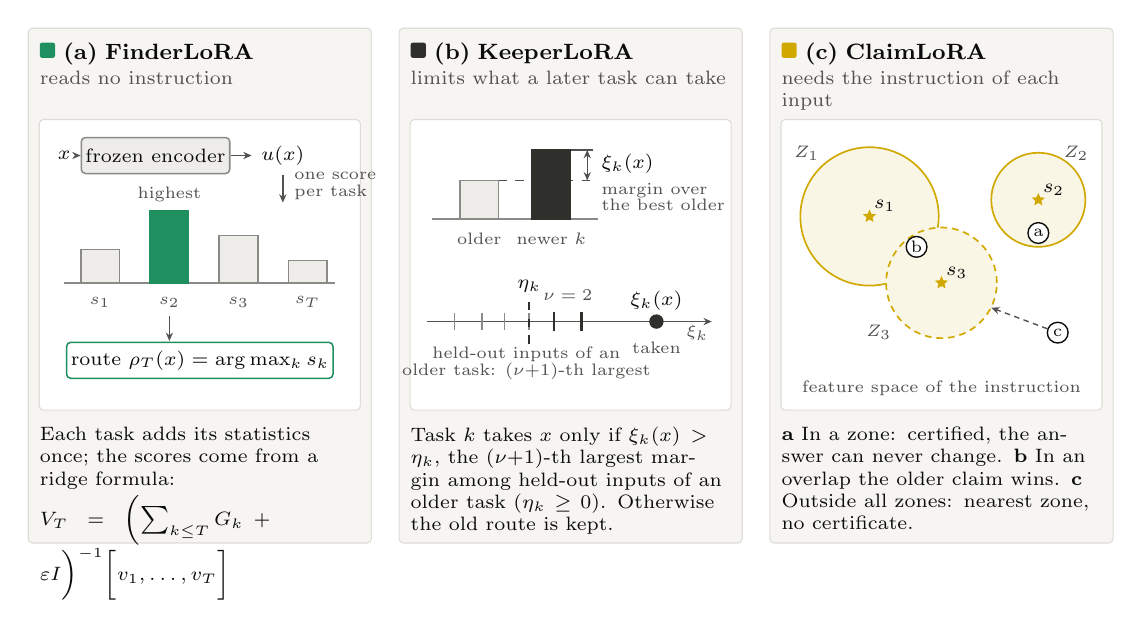
\begin{tikzpicture}[color=ink]
\def\W{124}\def\H{196}
\foreach \i in {0,1,2}{
  \fill[panelbg, draw=hair, line width=0.4pt, rounded corners=1.5pt] (\i*134,10) rectangle (\i*134+\W,\H);
  \fill[white, draw=hair, line width=0.4pt, rounded corners=1.5pt] (\i*134+4,58) rectangle (\i*134+\W-4,\H-33);
}
% ============ (a) FinderLoRA
\begin{scope}[shift={(0,0)}]
  \node[anchor=north west, text width=116pt, inner sep=0] at (4,\H-5)
    {\footnotesize\bfseries \chip{cfind}(a) \recog{}\\[1pt]\scriptsize\mdseries\color{ink2} reads no instruction};
  \node (ax) at (13,150) {$x$};
  \node[bb, minimum width=46pt] (enc) at (46,150) {frozen encoder};
  \node (au) at (92,150) {$u(x)$};
  \draw[flow] (ax) -- (enc); \draw[flow] (enc) -- (au);
  \draw[flow] (au.south) -- (92,133);
  \node[small, anchor=west, inner sep=0, align=left] at (96,139) {one score\\[-1pt]per task};
  \def\bl{104}
  \draw[line width=0.5pt, draw=muted] (13,\bl) -- (111,\bl);
  \foreach \xx/\hh/\lab in {26/12/{s_1},51/26/{s_2},76/17/{s_3},101/8/{s_T}}{
    \fill[bar] (\xx-7,\bl) rectangle (\xx+7,\bl+\hh);
    \node[small] at (\xx,\bl-7) {$\lab$};
  }
  \fill[cfind, draw=cfind, line width=0.5pt] (44,\bl) rectangle (58,\bl+26);
  \node[small] at (51,\bl+32) {highest};
  \node[box, draw=cfind, fill=white, minimum width=88pt] (route) at (62,76) {route $\rho_T(x)=\arg\max_k s_k$};
  \draw[flow] (51,\bl-12) -- (51,83);
  \node[anchor=north west, text width=116pt, inner sep=0, align=left] at (4,52)
    {\scriptsize Each task adds its statistics once; the scores come from a ridge formula:\\[1.5pt]
     \centering $V_T=\bigl(\sum_{k\le T}G_k+\varepsilon I\bigr)^{-1}\bigl[v_1,\dots,v_T\bigr]$};
\end{scope}
% ============ (b) KeeperLoRA
\begin{scope}[shift={(134,0)}]
  \node[anchor=north west, text width=116pt, inner sep=0] at (4,\H-5)
    {\footnotesize\bfseries \chip{ckeep}(b) \handicap{}\\[1pt]\scriptsize\mdseries\color{ink2} limits what a later task can take};
  \def\bl{127}
  \draw[line width=0.5pt, draw=muted] (12,\bl) -- (72,\bl);
  \fill[bar] (22,\bl) rectangle (36,\bl+14);
  \draw[dashed, line width=0.4pt, draw=ink2] (36,\bl+14) -- (70,\bl+14);
  \fill[ckeep, draw=ckeep, line width=0.5pt] (48,\bl) rectangle (62,\bl+25);
  \draw[line width=0.4pt, draw=ink2] (62,\bl+25) -- (70,\bl+25);
  \draw[<->, line width=0.5pt, draw=ink2] (68,\bl+14) -- (68,\bl+25);
  \node[small] at (29,\bl-7) {older};
  \node[small] at (55,\bl-7) {newer $k$};
  \node[anchor=west, inner sep=0] at (73,\bl+20) {$\xi_k(x)$};
  \node[small, anchor=west, inner sep=0, align=left] at (73,\bl+8) {margin over\\[-1pt]the best older};
  \def\al{90}
  \draw[->, line width=0.5pt, draw=ink2] (10,\al) -- (113,\al) node[anchor=north east, small, inner sep=1pt] {$\xi_k$};
  \foreach \p in {20,30,38,47,56,66}{ \draw[line width=0.5pt, draw=muted] (\p,\al-3) -- (\p,\al+3); }
  \draw[line width=0.9pt, draw=ckeep] (66,\al-3.5) -- (66,\al+3.5);
  \draw[line width=0.9pt, draw=ckeep] (56,\al-3.5) -- (56,\al+3.5);
  \draw[dashed, line width=0.5pt, draw=ckeep] (47,\al-8) -- (47,\al+10);
  \node[anchor=south, inner sep=0.5pt] at (47,\al+10) {$\eta_k$};
  \node[small, anchor=south] at (61,\al+4) {$\nu=2$};
  \fill[ckeep] (93,\al) circle (2.6pt);
  \node[anchor=south, inner sep=1pt] at (93,\al+3) {$\xi_k(x)$};
  \node[small, anchor=north] at (93,\al-4) {taken};
  \node[small, anchor=north, inner sep=0, align=center] at (46,\al-9) {held-out inputs of an\\[-1pt]older task: $(\nu{+}1)$-th largest};
  \node[anchor=north west, text width=116pt, inner sep=0, align=left] at (4,52)
    {\scriptsize Task $k$ takes $x$ only if $\xi_k(x)>\eta_k$, the $(\nu{+}1)$-th largest margin among held-out inputs of an older task ($\eta_k\ge 0$). Otherwise the old route is kept.};
\end{scope}
% ============ (c) ClaimLoRA
\begin{scope}[shift={(268,0)}]
  \node[anchor=north west, text width=116pt, inner sep=0] at (4,\H-5)
    {\footnotesize\bfseries \chip{cclaim}(c) \cert{}\\[1pt]\scriptsize\mdseries\color{ink2} needs the instruction of each input};
  \def\zf{cclaim!10}
  \fill[\zf, draw=cclaim, line width=0.6pt] (36,128) circle (25);
  \fill[\zf, draw=cclaim, line width=0.6pt] (97,134) circle (17);
  \fill[\zf, draw=cclaim, line width=0.6pt, dash pattern=on 2.4pt off 1.8pt] (62,104) circle (20);
  \foreach \cx/\cy in {36/128,97/134,62/104}{
    \node[star, star points=5, star point ratio=2.2, fill=cclaim, draw=none, inner sep=0, minimum size=5pt] at (\cx,\cy) {};
  }
  \node[anchor=south west, inner sep=0.5pt] at (37,129) {$s_1$};
  \node[anchor=south west, inner sep=0.5pt] at (98,135) {$s_2$};
  \node[anchor=south west, inner sep=0.5pt] at (63,105) {$s_3$};
  \node[small, anchor=south east, inner sep=0] at (18,148) {$Z_1$};
  \node[small, anchor=south west, inner sep=0] at (106,148) {$Z_2$};
  \node[small, anchor=north east, inner sep=0] at (44,89) {$Z_3$};
  % example inputs a, b, c
  \node[circle, draw=ink, fill=white, line width=0.5pt, inner sep=0pt, minimum size=7.5pt, font=\fontsize{6.5}{7}\selectfont] (pa) at (97,122) {a};
  \node[circle, draw=ink, fill=white, line width=0.5pt, inner sep=0pt, minimum size=7.5pt, font=\fontsize{6.5}{7}\selectfont] (pb) at (53,117) {b};
  \node[circle, draw=ink, fill=white, line width=0.5pt, inner sep=0pt, minimum size=7.5pt, font=\fontsize{6.5}{7}\selectfont] (pc) at (104,86) {c};
  \draw[->, dash pattern=on 2pt off 1.6pt, line width=0.5pt, draw=ink2] (pc) -- (80,95);
  \node[small] at (62,66) {feature space of the instruction};
  \node[anchor=north west, text width=116pt, inner sep=0, align=left] at (4,52)
    {\scriptsize \textbf{a} In a zone: certified, the answer can never change. \textbf{b} In an overlap the older claim wins. \textbf{c} Outside all zones: \mbox{nearest} zone, no certificate.};
\end{scope}
\end{tikzpicture}
\end{document}
